\documentclass[a4paper,10pt]{article}
\usepackage[utf8]{inputenc}
\usepackage[T1]{fontenc}
\usepackage[french]{babel}
\usepackage{graphicx}
\usepackage{amsmath}

\newcommand\tabA[1][0.5cm]{\hspace*{#1}}
\newcommand\tabB[1][1.5cm]{\hspace*{#1}}
\newcommand\tabC[1][2cm]{\hspace*{#1}}
\setlength{\parindent}{0cm}
\setlength{\parskip}{1ex plus 0.5ex minus 0.2ex}
\newcommand{\hsp}{\hspace{20pt}}
\newcommand{\HRule}{\rule{\linewidth}{0.5mm}}
% Title Page
\begin{document}
\begin{titlepage}
  \begin{sffamily}
  \begin{center}

    % Upper part of the page. The '~' is needed because \\
    % only works if a paragraph has started.
    
\includegraphics{./image/ua_v_couleur.jpg}
    
    \textsc{ UNIVERSIT\'{E} D'ANGERS \\ UFR INFORMATIQUE}\\[0.5cm]
    \textsc{ \\ Rapport de stage \\ Master 1 2016-2017 }\\[1.5cm]
    
    
\includegraphics{./image/logo-generique-SD.png}
    
    \textsc{UMR INSERM 1232 \\-Equipe Immunité Innée et Immunothérapie}\\[1cm]
     
    % Title
    \HRule \\[0.4cm]
    { \huge \bfseries ANALYSE TRANSCRIPTOMIQUE\\[0.4cm] }

    \HRule \\[2cm]

    % Author and supervisor
    \begin{minipage}{0.4\textwidth}
      \begin{flushleft} \large
        \large Présenté par : \\\textsc{RASOLONIAINA Marlino}
      \end{flushleft}
    \end{minipage}
    \begin{minipage}{0.4\textwidth}
      \begin{flushright} \large
        \emph{Tuteur :} M. Le \textsc{Tuteur}\\
        \emph{Chef d'équipe : } M. Chef \textsc{D’Équipe}
      \end{flushright}
    \end{minipage}

    \vfill

    % Bottom of the page
    {\large 12 Avril 2017 — 20 Juin 2017}

  \end{center}
  \end{sffamily}
\end{titlepage}
\newpage
\tableofcontents
\newpage
\section{INTRODUCTION :}
\section{ACQUISITION DES DONN\'{E}ES :}
\subsection{Les puces à ADN :}
La technologie qui prédomine est basée sur les puces à ADN.
  Une puce à ADN est constituée d'un support physique (le plus
  souvent une lame de verre) sur lequel sont déposées des molécules
  d'ADN correspondant à de petits fragments du génome (jusqu'à 40 000
  dépôts différents par puce). On recouvre la puce
  de la solution contenant la population d'ARN à étudier. Les ARN
  s'hybrident sur les fragments d'ADN complémentaires. La quantité d'ARN
  fixée reflète la concentration de cet ARN dans la solution. Il
  peut exister des biais systématiques dus à d'autres facteurs,
  tels que l'affinité des séquences ou l'efficacité du marquage. 
  \newline
 Pour des raisons pratiques, on utilise des ADNc plutôt que directement
  les ARN. Les ADNc sont marqués par un nucléotide radioactif ou
  un fluorochrome. Il est possible d'étudier simultanément plusieurs
  populations d'ADNc sur une même puce en utilisant des fluorochromes différents.
  La meilleure façon d'utiliser cette possibilité est de marquer
  de l'ADN génomique avec un fluorochrome, toujours le même. On
  obtient ainsi une référence stable au cours des années
  qui permet de mettre toutes les puces à la même échelle,
  quelle que soit leur origine. 
  \newline
  Un scanner mesure l'intensité du signal émis
  par l'ADNc hybridé au
  niveau de chaque dépôt. Parmi les valeurs que proposent les
  logiciels pour cette intensité, la plus fiable est la médiane de l'intensité des pixels car elle est moins sensible aux défauts de
  l'image (pixels sur-brillants par exemple). 
  \newline
  Les puces comportent généralement plusieurs
  dépôts
  identiques pour chaque gène. Cela simplifie le travail lorsqu'il faut
  repérer les aberrations dans la lecture des intensités puisqu'il
  suffit d'examiner les cas où les valeurs diffèrent beaucoup d'un
  dépôt à l'autre. Il s'agit le plus souvent d'un défaut
  physique sur la puce et il est facile d'éliminer la valeur aberrante.
  Dans le doute, on conserve la médiane des différentes mesures. 
\subsection{La technologie Illumina :}

\subsection{ Plan expérimental :}
\begin{center}
 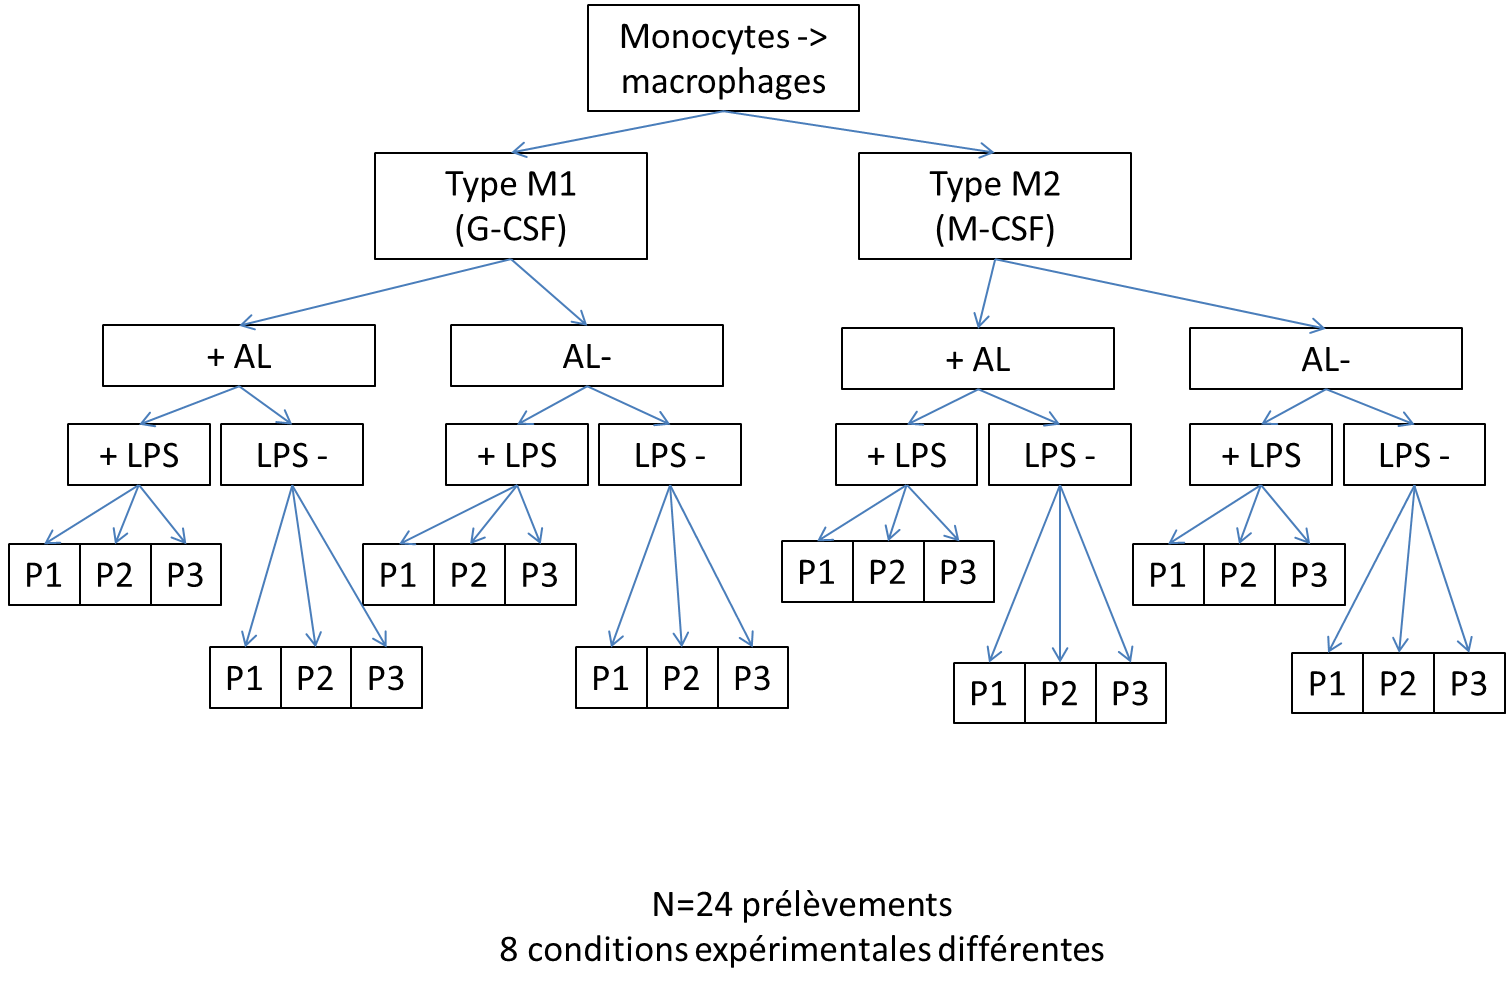
\includegraphics[scale=0.5]{./image/plan.png}
 % plan.png: 0x0 pixel, 300dpi, 0.00x0.00 cm, bb=
\end{center}
L’expression des gènes des macrophages a été analysée par des puces d’expression génique de technologie Illumina avec 48210 sondes pour chaque prélèvement.
Ce qui nous donne une matrice de données de dimmension (48210 x 24) avec les 24 prélèvements.
\[
\begin{pmatrix}

   a_{11} & \cdots & a_{1m} \\

   \vdots & \ddots &\vdots \\

   a_{n1} & \cdots & a_{nm} 

\end{pmatrix}
\]
\subsection{Les biais possibles :}

\section{DESCRIPTION DES DONN\'{E}ES :}
\subsection{ Decryptage et lecture :}
\subsection{ Données brutes :}
\begin{itemize}
 \item idat
 \item bgx
 \item sdf
 \item cfg
 \item Metrics.txt
\end{itemize}
\subsection{ Contrôle et qualité :}

\section{PR\'{E}TRAITEMENT DES DONN\'{E}ES :}
\subsection{Transformation :}
\subsection{Normalisation :}
\subsection{Filtrage :}

\section{ANALYSE DES DONN\'{E}ES DE TRANSCRIPTOME :}
\subsection{Gènes différentiellement exprimés :}
\subsection{Gènes co-exprimés :}

\section{INTERP\'{E}TATION :}
Caractérisation d’un ensemble de gènes
\begin{abstract}
\end{abstract}
\end{document}          
